\documentclass{ctexbeamer}
\usetheme{sjtubeamer}
\usetikzlibrary{math}
\tikzexternalize[prefix=cache/]
\begin{document}
\begin{frame}
  \frametitle{缓存插图}
  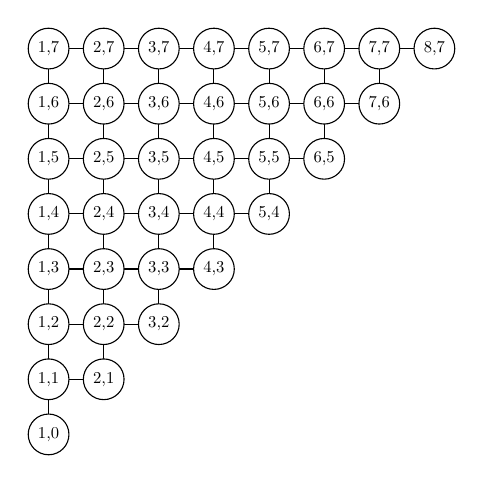
\begin{tikzpicture}[scale=0.7]
    \foreach \x in {1,...,7}{
        \foreach \y in {\x,...,7}{
            \draw (\x,\y-1)--(\x,\y);
            \draw (\x+1,\y)--(\x,\y);
          }
      }
    \foreach \x in {1,...,8}{
        \pgfmathparse{int(\x-1)}
        \foreach \y in {\pgfmathresult,...,7}{
            \node[draw,circle,fill=white,scale=0.6]
            at (\x,\y) {\x,\y};
          }
      }
  \end{tikzpicture}
\end{frame}
\end{document}